\chapter{Data Preparation and Model Training}\label{chap:training}

\section{Introduction}
Ideally, the Sim Translator should be trained with paired waveforms ($X, X'$) where $Y=Y'$ for each pair. In reality, collecting such a paired dataset is highly challenging. While we can simulate $\mathcal{T}_{Source}$ from an arbitrary $\mathcal{D}_{Source}$, obtaining a corresponding $\mathcal{T}_{Target}$ such that $\mathcal{D}_{Source} = \mathcal{D}_{Target}$ is difficult without precise knowledge of $P(X'|Y')$. Consequently, training must be conducted on unpaired datasets, where $\mathcal{D}_{Source} \neq \mathcal{D}_{Target}$. The CycleGAN framework~\cite{CycleGAN} provides a way to train the Sim Translator using adversarial losses even when paired data are unavailable

In this chapter, we first outline the detector data collection process, then describe the simulation approach, and finally detail the adversarial training of the network using CycleGAN.

\section{Data selection}

The LEGEND collaboration characterizes newly produced HPGe detectors at Oak Ridge National Laboratory (ORNL). We use characterization data from a LEGEND Inverted-Coaxial Point-Contact (ICPC) detector, V06643A, manufactured by ORTEC. The detector was mounted in a “PopTop” configuration, surrounded by lead shielding, and placed in a concrete alcove to reduce external background. The data contained a flood Thorium-232 source on top of the detector. Signals from the detector were digitized using a FlashCam digitizer, and the \texttt{pygama} package~\cite{pygama} was used to convert FlashCam output to LEGEND LH5-format HDF5 files, and to calibrate the event energies from ADC units to keV. The energies were then corrected for charge trapping. The left panel of Fig.~\ref{fig:eng_spec} shows the final energy spectrum obtained from the detector.


The escape peaks in spectrum are created from pair production events from a high energy photon. In this process, the incident photon generates an electron-positron pair. The electron is collected by the detector, while the positron quickly annihilates, producing two additional gamma-ray photons. If all secondary gamma rays are fully absorbed within the detector, their combined energy yields a characterized peak in the energy spectrum, the Full Energy Peak (FEP).


If one of the annihilation gamma rays leaves the detector without depositing its energy, the spectrum shows a Single Escape Peak (SEP). This scenario results in a multisite (MS) event because the signal comprises of two distinct interactions within the detector: the collection of the pair-produced electron and the absorption of one of the two gamma rays. If both gamma rays escape the detector without interaction, a double escape peak (DEP) is observed. This situation corresponds to a single site (SS) event since the only interaction that contributes to the signal is the collection of the pair-produced electron. Tl-208 is part of the decay chain of $^{228}$Th, and produces an FEP at $2614.53$ keV. Given the mass of the electron is $511$ keV, the SEP peak occurs at $2103.53$ keV and the DEP peak at $1592.53$ keV. 


\begin{figure}%[htb!]
  %[trim={left bottom right top},clip]
    \centering
    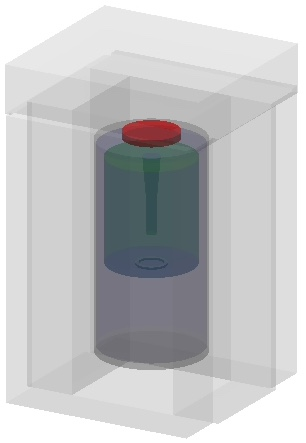
\includegraphics[width=0.4\linewidth]{ch7/figs/shielding.jpeg}
    \caption{The simulation geometry of the ORNL characterization setup, showing the detector in green, the source in red, the aluminum holder in light blue, and the lead shielding in light grey.}
   \label{fig:g4simple_setup}
\end{figure}


\begin{figure}%[htb!]
\centering
  %[trim={left bottom right top},clip]
    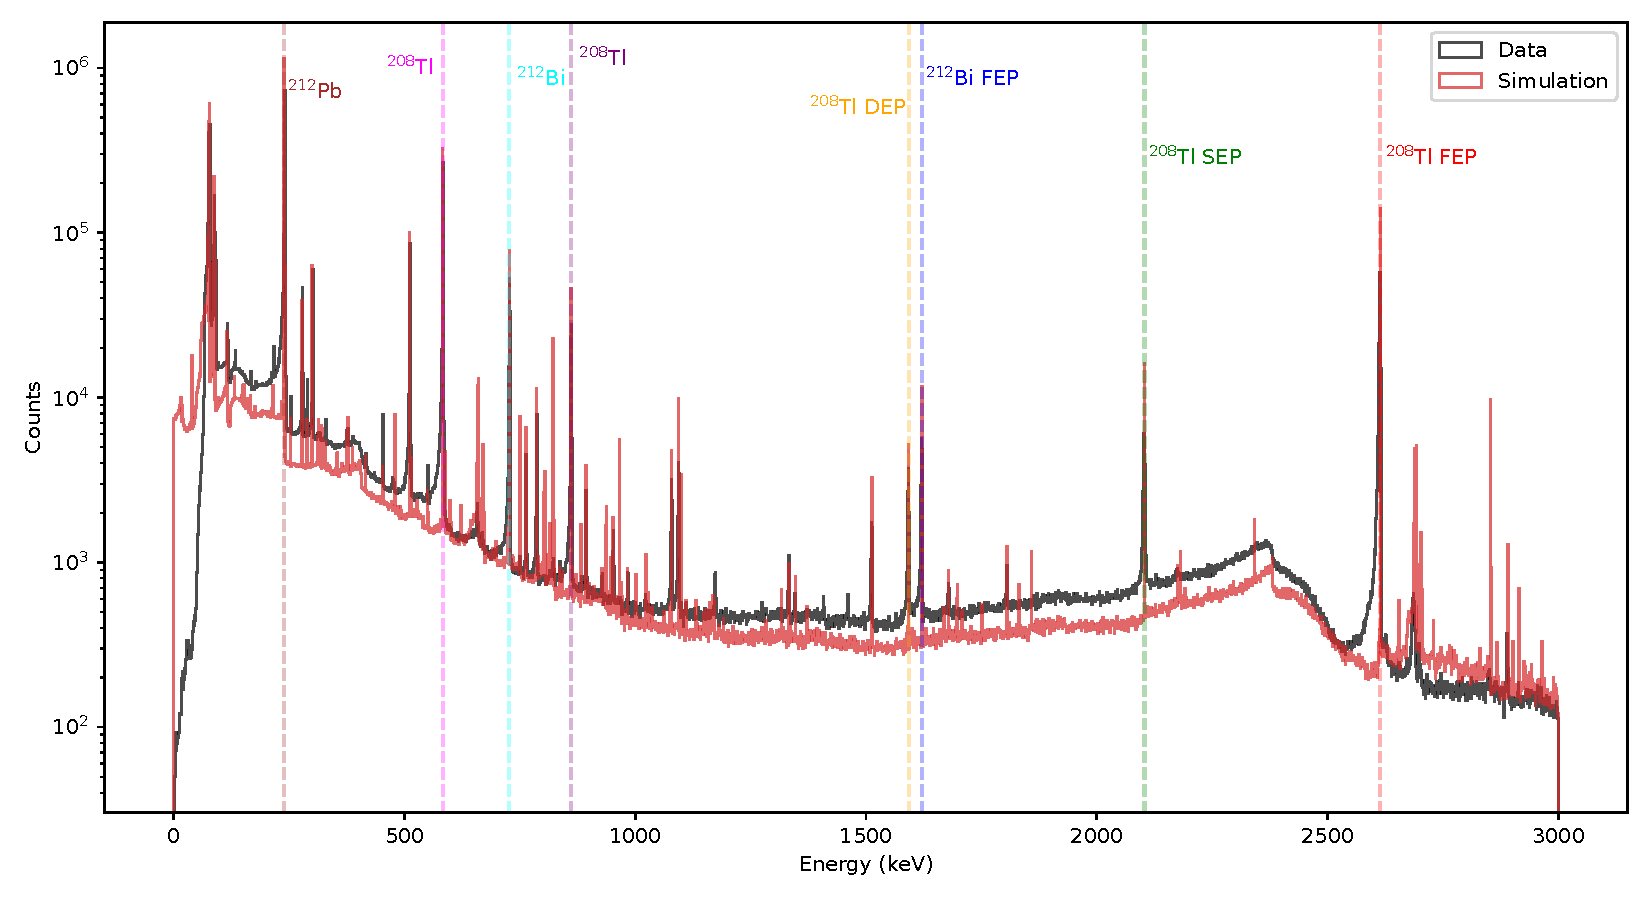
\includegraphics[width=0.99\linewidth,trim={0pc 0pc 0pc 0pc},clip]{ch7/figs/energy_spectrum_comparison.pdf}
    \caption{Measured energy spectrum from a $^{228}$Th source compared to the Monte Carlo simulation results. Key peaks from $^{228}$Th source are labeled.}
   \label{fig:eng_spec}
\end{figure}

\section{Simulations}


\begin{figure}[htb!]
  %[trim={left bottom right top},clip]
    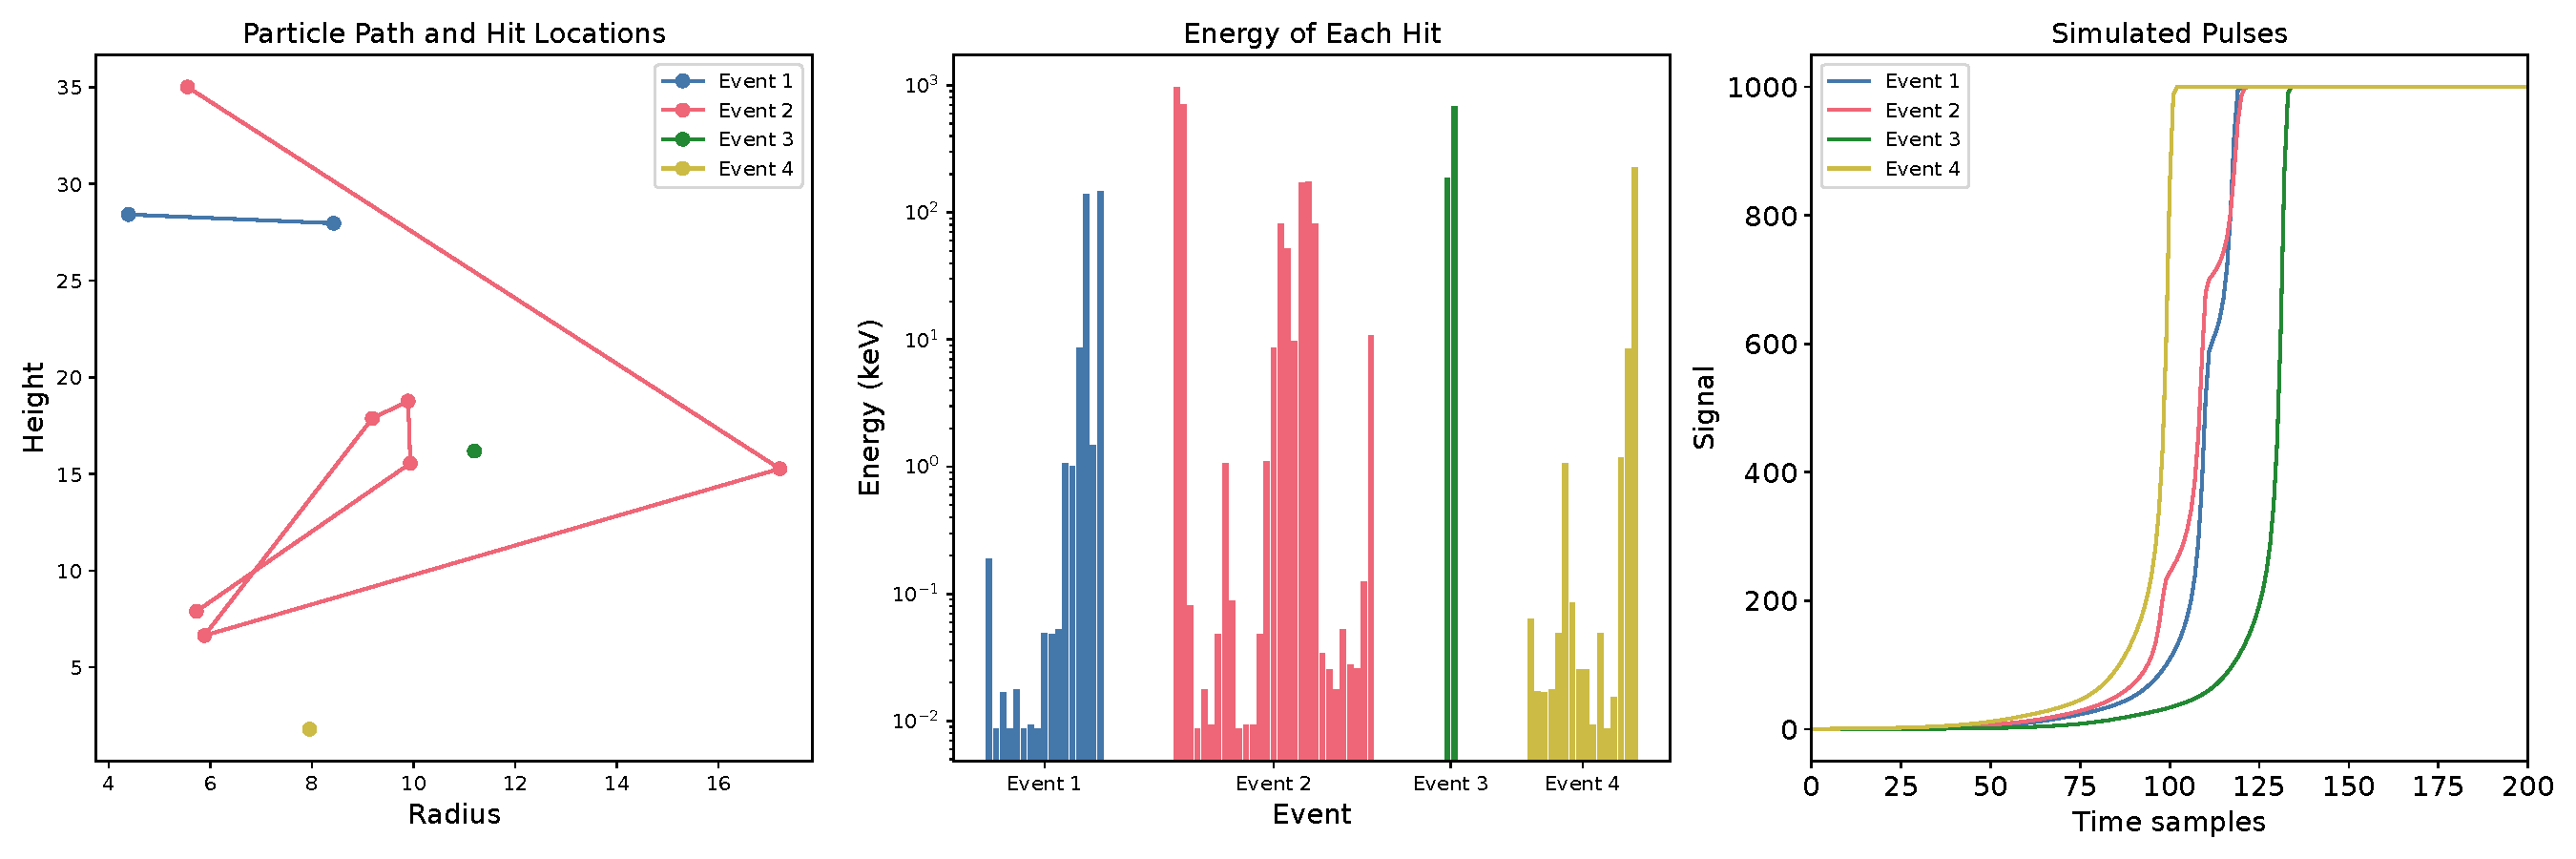
\includegraphics[width=0.99\linewidth,trim={1pc 0pc 1pc 0pc},clip]{ch7/figs/hit_sims.pdf}
    \caption{(Left) Hit locations for each event. (Right) Energy-weighted waveforms for the corresponding events. Hits produced using \texttt{Geant4} simulations and waveforms generated using \texttt{siggen} software.}
   \label{fig:eng_dep_sim}
\end{figure}


Geant4 is a Monte Carlo-based toolkit that can simulate the passage of particles through matter. We designed a simple Geant4 setup geometry to simulate events in the setup of ORNL characterization. The setup in  Geant4 shown in Fig. \ref{fig:eng_spec} This includes a Germanium detector, a radioactive source, Aluminum PopTop cryostat holder, surrounded by lead shielding. We simulated 100 million $^{228}$Th decay events originating from the source and recorded their energy depositions within the germanium detector. Given the location of energy deposition inside the detector, we used Siggen simulations to generate waveforms for hits in DEP, SEP and FEP energies.


Waveforms for multi-site events are creating by energy weighted summing of individual hits waveforms. Fig. ~\ref{fig:eng_dep_sim} shows the simulation process for few events. The left panel depicts the hits locations of particles for the events. Event 3 and Event 4 are effectively single-sited, as the energy depositions occur very close to each other and thus produces a single sited events. In Event 1, the energy depositions result in two primary sites, giving rise to a two-sited waveform. Event 2 features a trace of energy deposition localized to three regions, classifying it as a three-sited event. Event 3 and 4 have different drift times due being deposited at different distance from the point contact.

\section{Post Processing}

Normalizing and align are crucial for training the network. The sim waveforms are already normalized between 0 and 1.The raw data waveforms are normalized by dividing with the $80\%$ of the average of the last five samples. Then the waveform is shifted so that the average of the first 200 samples is zero. This ensure that the all the waveforms have their RC decay tails and baseline aligned. Then we used $99.9\%$ rise time to align the waveform. We found this method was more effective in training the network than aligning by zero time point. The waveforms are padded to ensure there are 400 samples on both sides of $99.9\%$ rise time. The tail slope $\tau$ is calculated by the slope of a linear fit of the logarithm of the last 300 waveform samples. Events with poor fit quality $\chi^2$ or anomalous $\tau$ are used to identify pile-up waveforms and remove them from the training. Fig. \ref{ch7:figs:in_out} shows the processed data and sim waveforms.

\begin{figure}[!htb]
    % \hspace{0.05\linewidth}
    %[trim={left bottom right top},clip]
    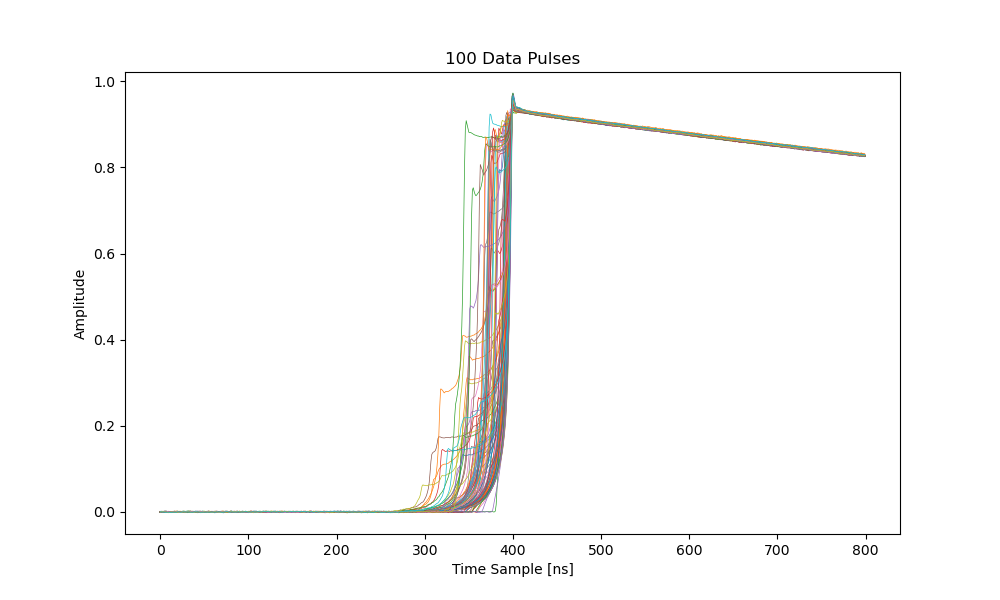
\includegraphics[width=0.95\linewidth,trim={0pc 0cm 0pc 1cm},clip]{ch7/figs/all_data_pulses.png}
    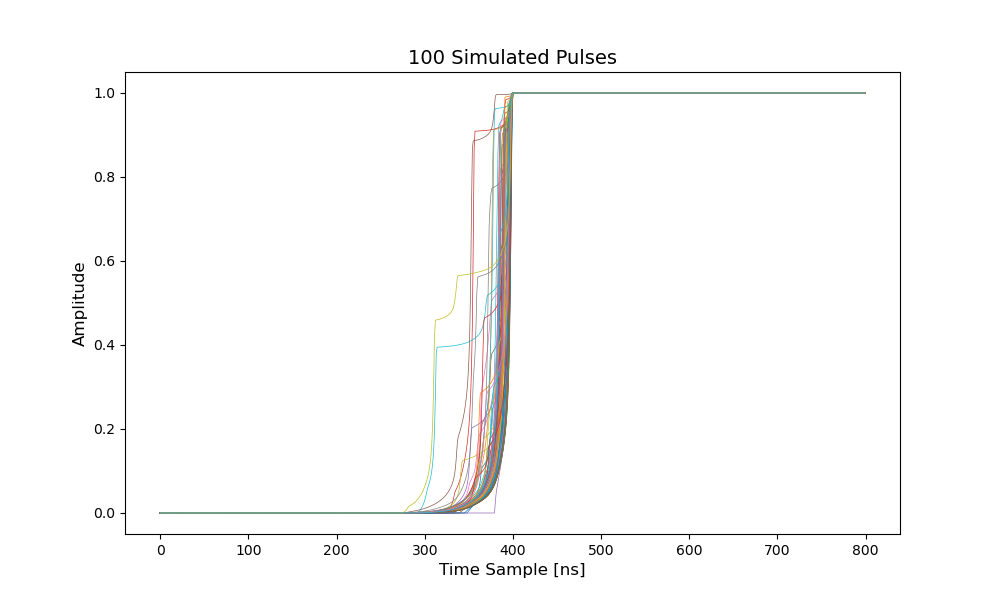
\includegraphics[width=0.95\linewidth,trim={0pc 0cm 0pc 1cm},clip]{ch7/figs/all_simulated_pulses.png}
    \caption{Input data and simulated waveforms. The waveforms are aligned by $99.9\%$ rise time. Data pulses are normalized by aligning the tail and baselines.}
   \label{ch7:figs:in_out}
\end{figure}


\section{Network Training}

The training and validation of CPU-Net are conducted in PyTorch~\cite{pytorch}. We construct two networks an Sim Translator~ $\Lambda$ and an Inverse Sim Translator $\bar{\Lambda}$, both with PU-Net structure. We then construct two RNN discriminator networks sim discriminator $\delta_{S}$ and data discriminator $\delta_{T}$ for the source and target waveforms, respectively. Figure~\ref{fig:network_training} shows the overall training process.
\clearpage
\begin{figure}[htb!]
    % \hspace{0.05\linewidth}
    %[trim={left bottom right top},clip]
    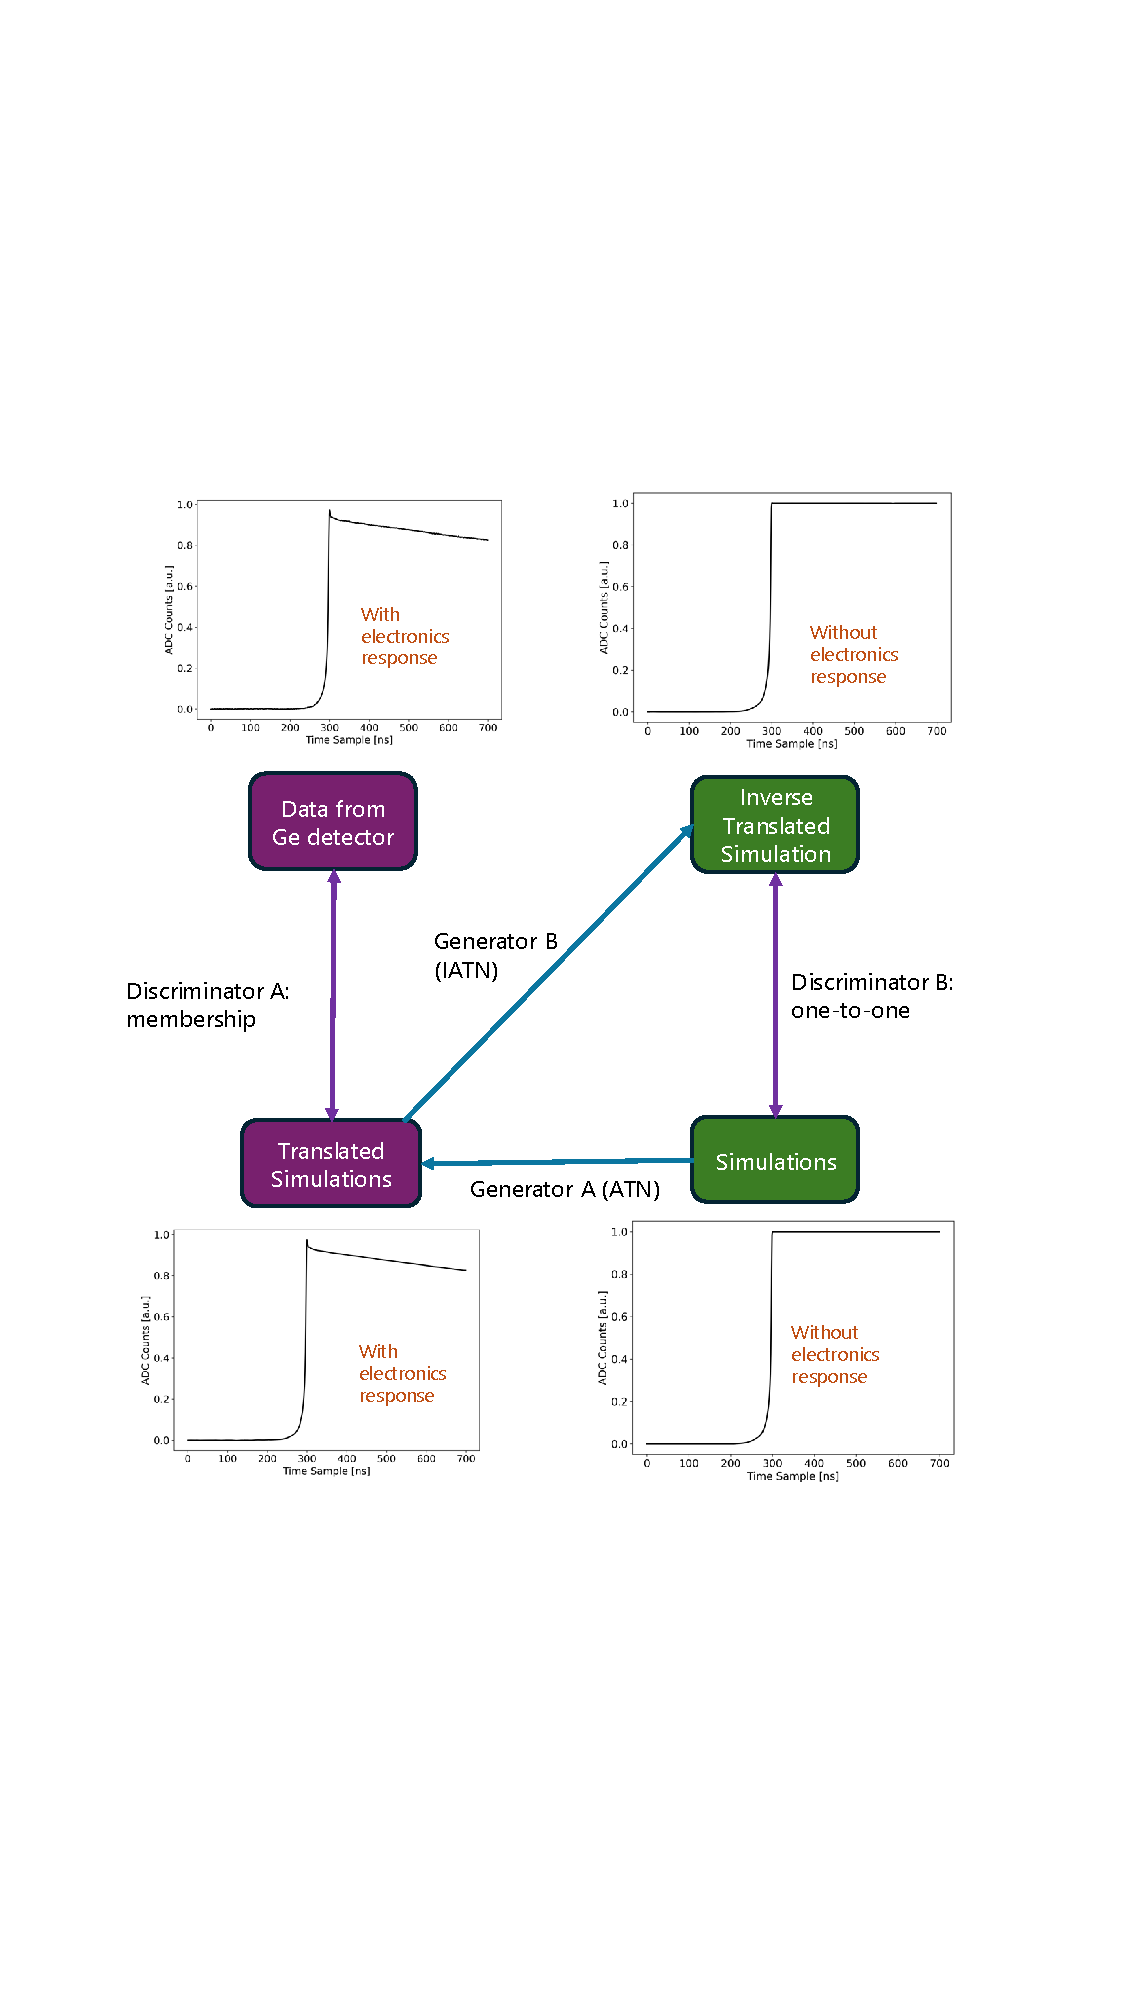
\includegraphics[width=0.99\linewidth,trim={5pc 20pc 6.5pc 19pc},clip]{ch7/figs/cycle_gan_training.pdf}
    \caption{Training in CPU net. Generator A transfers sim to data while Generator B transfers sim to data. Discriminator A differentiates data like waveform from Generator A from data. Discriminator B differentiates sim like waveform from Generator B from simulations.}
   \label{fig:network_training}
\end{figure}


When training the network, a simulated waveform $X$ is first fed to $\Lambda$ to produce a translated waveform $\Lambda(X)$. The discriminator $\delta_{T}$ attempts to distinguish $\Lambda(X)$ from real data waveforms while $\Lambda(X)$ tries to “fool” $\delta_{T}$. Then $\Lambda(X)$ is fed to $\bar{\Lambda}$ to translate back to $\mathcal{X}$ space by $\bar{\Lambda}(\Lambda(\mathcal{X}))$. A second discriminator $\delta_{S}$ attempts to distinguish $\bar{\Lambda}(\Lambda(\mathcal{X}))$ from $\mathcal{X}$ while $\bar{\Lambda}$ attempts to ``fool'' $\delta_{S}$. The $\mathcal{X}\rightarrow{}\Lambda(\mathcal{X})\rightarrow{}\bar{\Lambda}(\Lambda(\mathcal{X}))$ translation path is termed the forward cycle. The same process is performed in the other direction, starting with the detector waveform, $\mathcal{X}'\rightarrow{}\bar{\Lambda}(\mathcal{X}')\rightarrow{}\Lambda(\bar{\Lambda}(\mathcal{X}'))$ and called backward cycle.

\section{Loss Functions}
$L_{\mathrm{Identity}}$ ensures that the Sim Translator preserves its shape when an actual detector waveform $X'$ is fed into $\Lambda$, shown in Eq. \ref{eq:loss_ided}. The cycle-consistent loss in Eq. \ref{eq:loss_cyc} ensures the circular translation path preserves the original waveform shape, and the GAN loss Eq. \ref{eq:loss_gan} calculates the loss associated with ``fooling'' the discriminator. A specialized L1 loss is used for $L_{\mathrm{Identity}}$, $L_{\mathrm{Cycle}}$, $L_{\mathrm{Advesarial}}$ that emphasizes different parts of the waveform by assigning them varying weights. It's particularly designed to give more importance to the rising and falling edges of the waveform, which are critical for accurate waveform shape analysis. Binary Cross-Entropy Loss is used for the discriminator $\delta_{T}$.

\begin{equation}\label{eq:loss_ided}
    L_{\mathrm{Identity}} = |X' - \Lambda(X')|
\end{equation}
\begin{equation}\label{eq:loss_cyc}
    L_{\mathrm{Cycle}} = |X - \bar{\Lambda}(\Lambda(X))|
\end{equation}
\begin{equation}\label{eq:loss_gan}
    L_{\mathrm{Adversarial}} = E_{\mathcal{X'}}\log(\delta(X')) - E_{\Lambda(\mathcal{X})}\log(1 - \delta(\Lambda(X)))
\end{equation}

An additional three complementary losses are defined for the detector waveform translation path. Therefore, a total of six losses are optimized simultaneously for the generators and two for the discriminators. AdamW~\cite{adam_w_paper} optimizers are used for all losses. We trained the CPU-Net on 110,000 FEP waveforms. A linear learning rate decay begins at iteration 1000 and reaches zero at the final iteration. Table \ref{ch8:tab:loss_summary}

\begin{table}%[ht!]
\centering
\renewcommand{\arraystretch}{1.5} % Adjust row height for readability
\setlength{\tabcolsep}{2.0pt} % Adjust column spacing
\begin{tabular}{|p{0.18\linewidth}|p{0.39\linewidth}|p{0.22\linewidth}|p{0.15\linewidth}|}
\hline
Loss                & Calculation                             & Type of Loss                                  & Optimizer   \\ \hline
Identity Losses    & Data - ATN(Data)                                & \multirow{3}{=}{Custom L1 Loss} & \multirow{8}{=}{Optimizer 1} \\
                             & Sim - IATN(Data)                                 &                                                       &                       \\ \cline{1-3}
Cycle Losses        & Data – ATN(IATN(Data))                         & \multirow{3}{=}{Custom L1 Loss} &                       \\
                             & Sim – IATN(ATN(Sim))                          &                                                       &                       \\ \cline{1-3}
Generator Losses    & Disc B (IATN(Data))                              & \multirow{2}{=}{Binary Cross Entropy}                &                       \\
                             & Disc A (ATN(Sim))                              &                                                       &                       \\ \hline
Discriminator A     & {[Disc A(Data) - 1]} + {[Disc A(Sim) - 0]}        &  Binary Cross Entropy                                & Optimizers 2 \\ \hline
 Discriminator B    & {[Disc B(Sim) - 1]} + {[Disc B(Data) - 0]}        &   Binary Cross Entropy                                &   Optimizers 3             \\ \hline
\end{tabular}
\caption{Overview of Loss Calculations, Loss Types, and Optimizers.}
\label{ch8_tab_loss_summary}
\end{table}



To prevent overfitting during training, weight decay is applied to the optimizers so that it penalizes the large weights and encourages generalization. Gradient clipping is applied, limiting the norm of gradients during training and preventing exploding gradients, particularly in layers of the U-Net.

It was found that the discriminator typically overpowers the generator since the generator has a more complex task of generating waveforms while maintaining the cycle and identity consistency, and also fooling the discriminator. To balance this, we introduce a hyperparameter for the number of intervals after which the discriminator is updated. This allowed the generator enough steps to adapt to changes in the discriminator without destabilizing the adversarial process.

Combining all these, we obtain the Cyclic Positional U-Net~(CPU-Net) for Ad-hoc waveform shape simulation. The trained CPU-Net generates both a Sim Translator and an Inverse Sim Translator, which enables bidirectional translation between the simulation and data domains. The Sim Translator is the primary focus of this work, but the Inverse Sim Translator can also enhance analysis by refining waveform reconstruction. 

\section{Hyperparameter Tuning}

\begin{table}%[htb!]
\centering
\renewcommand{\arraystretch}{1.5} % Adjust row height for readability
\setlength{\tabcolsep}{2pt} % Adjust column spacing
\begin{tabular}{|p{0.18\linewidth}|p{0.12\linewidth}|p{0.65\linewidth}|}
\hline
\textbf{Hyperparameter}       & \textbf{Value} & \textbf{Description} \\ \hline
batch\_size          & 32             & Number of pulses used in one training iteration. \\ \hline
baseline\_len        & 200            & Number of samples assigned to baseline portion of the waveform. \\ \hline
rising\_edge\_len    & 250            & Number of samples assigned to the rising edge of the waveform. \\ \hline
tail\_len            & 350            & Number of samples assigned to the RC decay tail of the waveform. \\ \hline
baseline\_weight     & 3.0            & Weight given to baseline portion of the waveform in the loss. \\ \hline
ris\_edge\_weight    & 10.0           & Weight given to rising edge portion of the waveform in the loss. \\ \hline
tail\_weight         & 7.0            & Weight given to RC decay tail portion of the waveform in the loss. \\ \hline
iters                & 7000           & Maximum number of iterations for training. \\ \hline
decay                & 1000           & Iteration at which learning rate starts to decay. \\ \hline
lrate\_gen           & $1 \times 10^{-3}$ & Learning rate for the generator networks. \\ \hline
lrate\_disc          & $1 \times 10^{-3}$ & Learning rate for the discriminator networks. \\ \hline
cyc\_loss\_weight    & 20             & Weight of the cycle consistency losses.  \\ \hline
iden\_loss\_weight   & 5              & Weight of the identity loss. \\ \hline
gan\_loss\_weight    & 9              & Weight of the generator loss. \\ \hline
max\_grad\_norm      & 100            & Maximum gradient norm for gradient clipping. \\ \hline
w\_decay             & $1 \times 10^{-4}$ & Weight decay in the optimizers. \\ \hline
n\_disc\_iters       & 30             & Number of iterations after which the discriminators are updated. \\ \hline
\end{tabular}
\caption{Hyperparameters used for CPU-Net training.}
\label{tab:hyperparameters}
\end{table}


Table \ref{tab:hyperparameters} shows the hyperparameters used in the training. Together these parameters enable price fine-tuning CPU-Net training to get the right balance during training. A single training takes about 1 GPU hour on a NVIDIA A100 GPU.